\subsection{\large{Развертывание приложения}}
\addcontentsline{toc}{subsection}

Помимо программной реализации необходимо уделить внимание вопросам развертывания приложения.
Gitlab CI/CD является инструментом, используемым в компании для непрерывной интеграции и развертывания.
Он предоставляет большой набор возможностей для развертывания приложения.
Код системы хранится в монорепозитории.
Это сделано с целью повышения прозрачности развертывания.

Главным объектом в системе Gitlab CI/CD является Pipeline.
Pipeline состоит из Stage, где каждый Stage состоит из Job.
Pipeline -- это верхнеуровневый элемент набора операций,
который будет применяться к актуальной кодовой базе.

Правила развертывания в Gitlab CI/CD представляют собой Directed Acyclic Graph(DAG).
Stage выполняются строго последовательно, но между Job-ами можно устанавливать зависимости.

Пример зависимостей в Pipeline можно увидеть на рисунке ниже(см. рис\ref{pic:implementation__deployment-dependencies}).
\begin{figure}[H]
	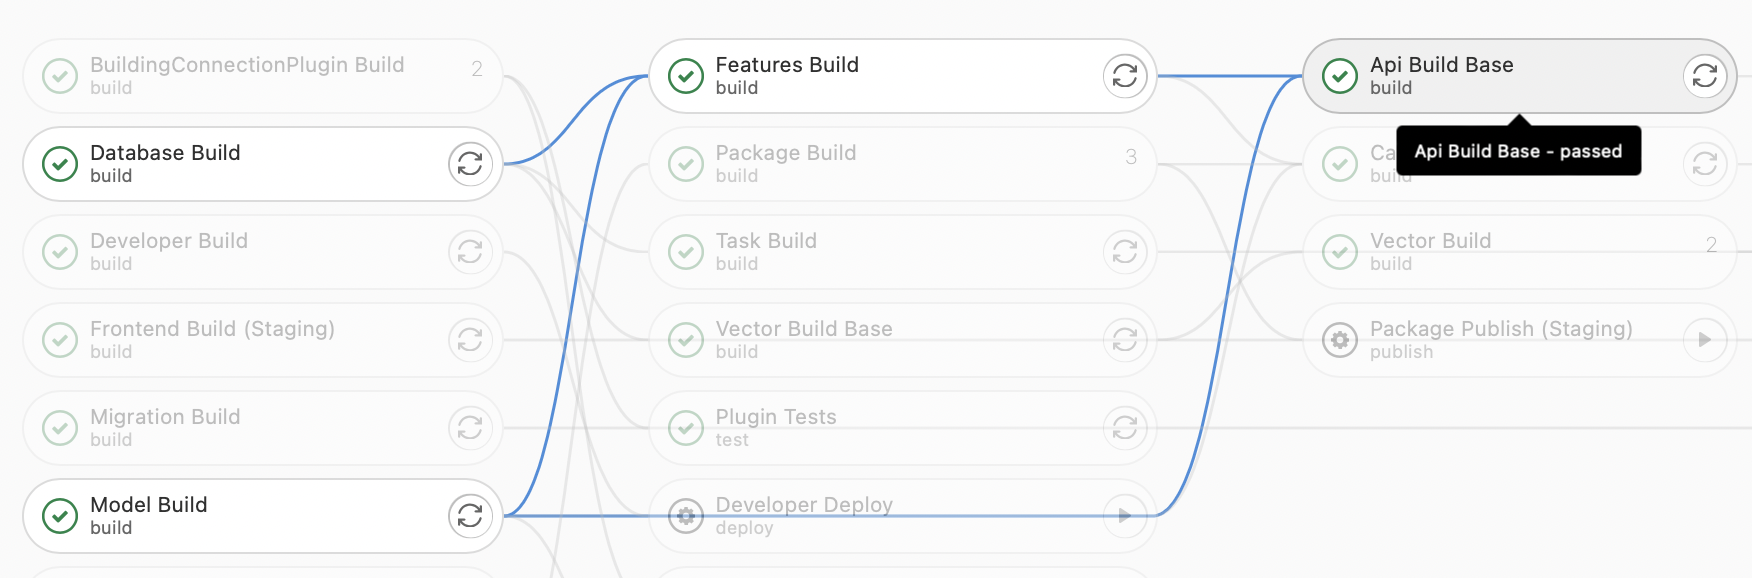
\includegraphics[width=\textwidth]{implementation/pictures/deployment/dependencies}
	\caption{Зависимости в Pipeline в Gitlab CI/CD}
	\label{pic:implementation__deployment-dependencies}
\end{figure}
\vskip 10mm

\noindent \textbf{Динамические окружения}

Gitlab CI/CD имеет возможность создания, как статических окружений, так и динамических.
Статические окружения представляют являются теми, с которыми взаимодействуют пользователи.
В нашем случае это \textit{staging} и \textit{production}.
То динамические окружения -- это отличное решение для изолированного тестирования нового функционала
отдельно от окружений, с которыми взаимодействуют пользователи. Именно они позволяют развернуть
изолированный прототип системы путем нажатия одной кнопки в интерфейсе.
Пример окружений можно увидеть на рисунке ниже(см. рис\ref{pic:implementation__deployment-environment}).
\begin{figure}[H]
	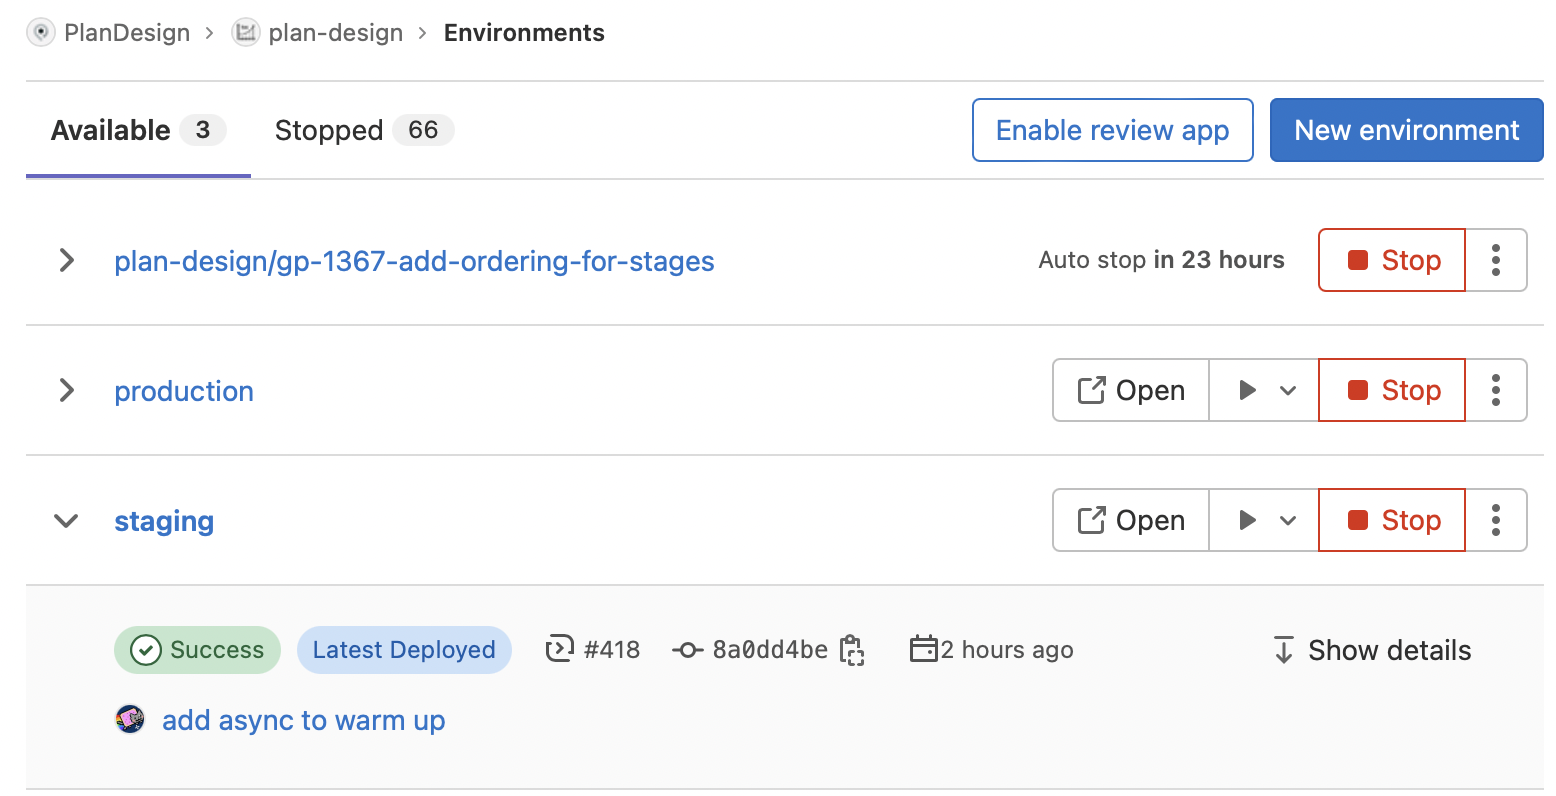
\includegraphics[width=\textwidth]{implementation/pictures/deployment/environment}
	\caption{Пример динамических окружений}
	\label{pic:implementation__deployment-environment}
\end{figure}
\vskip 10 mm

\noindent \textbf{Структура файлов CI/CD}

Все правила развертывания и сборки описываются в файле \textit{.gitlab-ci.yml},
его название и местоположение может быть изменено на любое другое в настройках репозитория.

Сложную конфигурацию CI/CD можно разбить на несколько разных логических компонент, поместив каждую из них
в отдельный файл.
С целью упрощения поддержки и добавления новых правил развертывания предлагается следующая структура файлов.

\dirtree{%
.1 gitlab-ci.
.2 stage1.
.3 services.
.4 service1.yml.
.4 service2.yml.
.4 service3.yml.
.3 main.yml.
.2 stage2.
.3 services.
.4 service1.yml.
.4 service3.yml.
.4 service7.yml.
.3 main.yml.
.2 stage3.
.3 services.
.4 service2.yml.
.4 service3.yml.
.3 main.yml.
.1 main.yml.
}
\vskip 5mm

Данная структура является иерархической.
Корневая директория называется \textit{gitlab-ci}. В корневой директории находится файл
\textit{gitlab-ci/main.yml}
(см. листинг\ref{lst:implementation__deployment_main_yml}),
внутри которого содержатся на верхнеуровневые файлы для каждого \textit{Stage}.
В директории каждого \textit{Stage} находится файл \textit{main.yml} (см. листинг\ref{lst:implementation__deployment_main_stage_yml})
который содержит включения на файлы
с описанием конфигурации для отдельного сервиса на этом этапе.

\lstinputlisting[
    caption={Пример кода \textbf{gitlab-ci/main.yml}},
    captionpos=b,
    label={lst:implementation__deployment_main_yml}
]{implementation/listings/deployment/main.yml}
\vskip 5mm

\lstinputlisting[
    caption={Пример кода \textbf{gitlab-ci/stage1/main.yml}},
    captionpos=b,
    label={lst:implementation__deployment_main_stage_yml}
]
{implementation/listings/deployment/main_stage.yml}
\vskip 5mm
